% ============================================================
% Xi Yin, Aspects of Two-Dimensional Conformal Field Theories
%   (PoS(TASI2017)003) 中译片段
% 第 5 章下半：5.2 节续文、5.3 节、5.4 节；第 6 章总结；致谢
% 底本：PDF 第 41--50 页（原书页码 40--49）
% 图 17--21；公式 (5.23)--(5.48)；停止于 References 标题之前
% ============================================================

% ===== 原书 p.40（PDF 41）：5.2 节续文，不重复小节标题 =====

数值上，我们可以用 $P_N v$ 近似 $v$，其中 $P_N$ 是到由 $p_{0,0}$ 与奇 $n+m$ 的 $p_{n,m}$ 张成的子空间上的正交投影。于是，$P_N v$ 可直接由线性方程组
\begin{equation}
  \label{eq:5-23}
  \begin{aligned}
    \langle v_N, p_{0,0}\rangle &= 1,\\
    \langle v_N, p_{m,n}\rangle &= 0,
      \quad m,n\ge 0,\ \text{odd } m+n\le N,
  \end{aligned}
\end{equation}
解出，并得到近似谱函数 $f_N(\Delta_*) = \langle P_N v,\theta(\Delta_*-\Delta)\rangle$。图~\ref{fig:16} 给出两个例子；可以看到 $f_N(\Delta_*)$ 随 $N$ 增大而稳定，并收敛到 Liouville 谱函数。

% [Tutor Note: 段首把基函数写作 $p_{n,m}$，(5.23) 中却写成 $p_{m,n}$；由于条件 $m,n\ge0$ 与奇 $m+n\le N$ 对 $m,n$ 对称，两者指同一族基函数，原文混用不影响线性方程组。]

与形如 $\langle\phi_1\phi_2\bar\phi_2\bar\phi_1\rangle$ 的混合关联子的类似结果一起，数值所提示的“$c>1$ 的 CFT 若只含标量 Virasoro 原初则谱函数唯一”这一性质，将意味着唯一具有该性质的 CFT 是 Liouville 理论。

\begin{figure}[htbp]
  \centering
  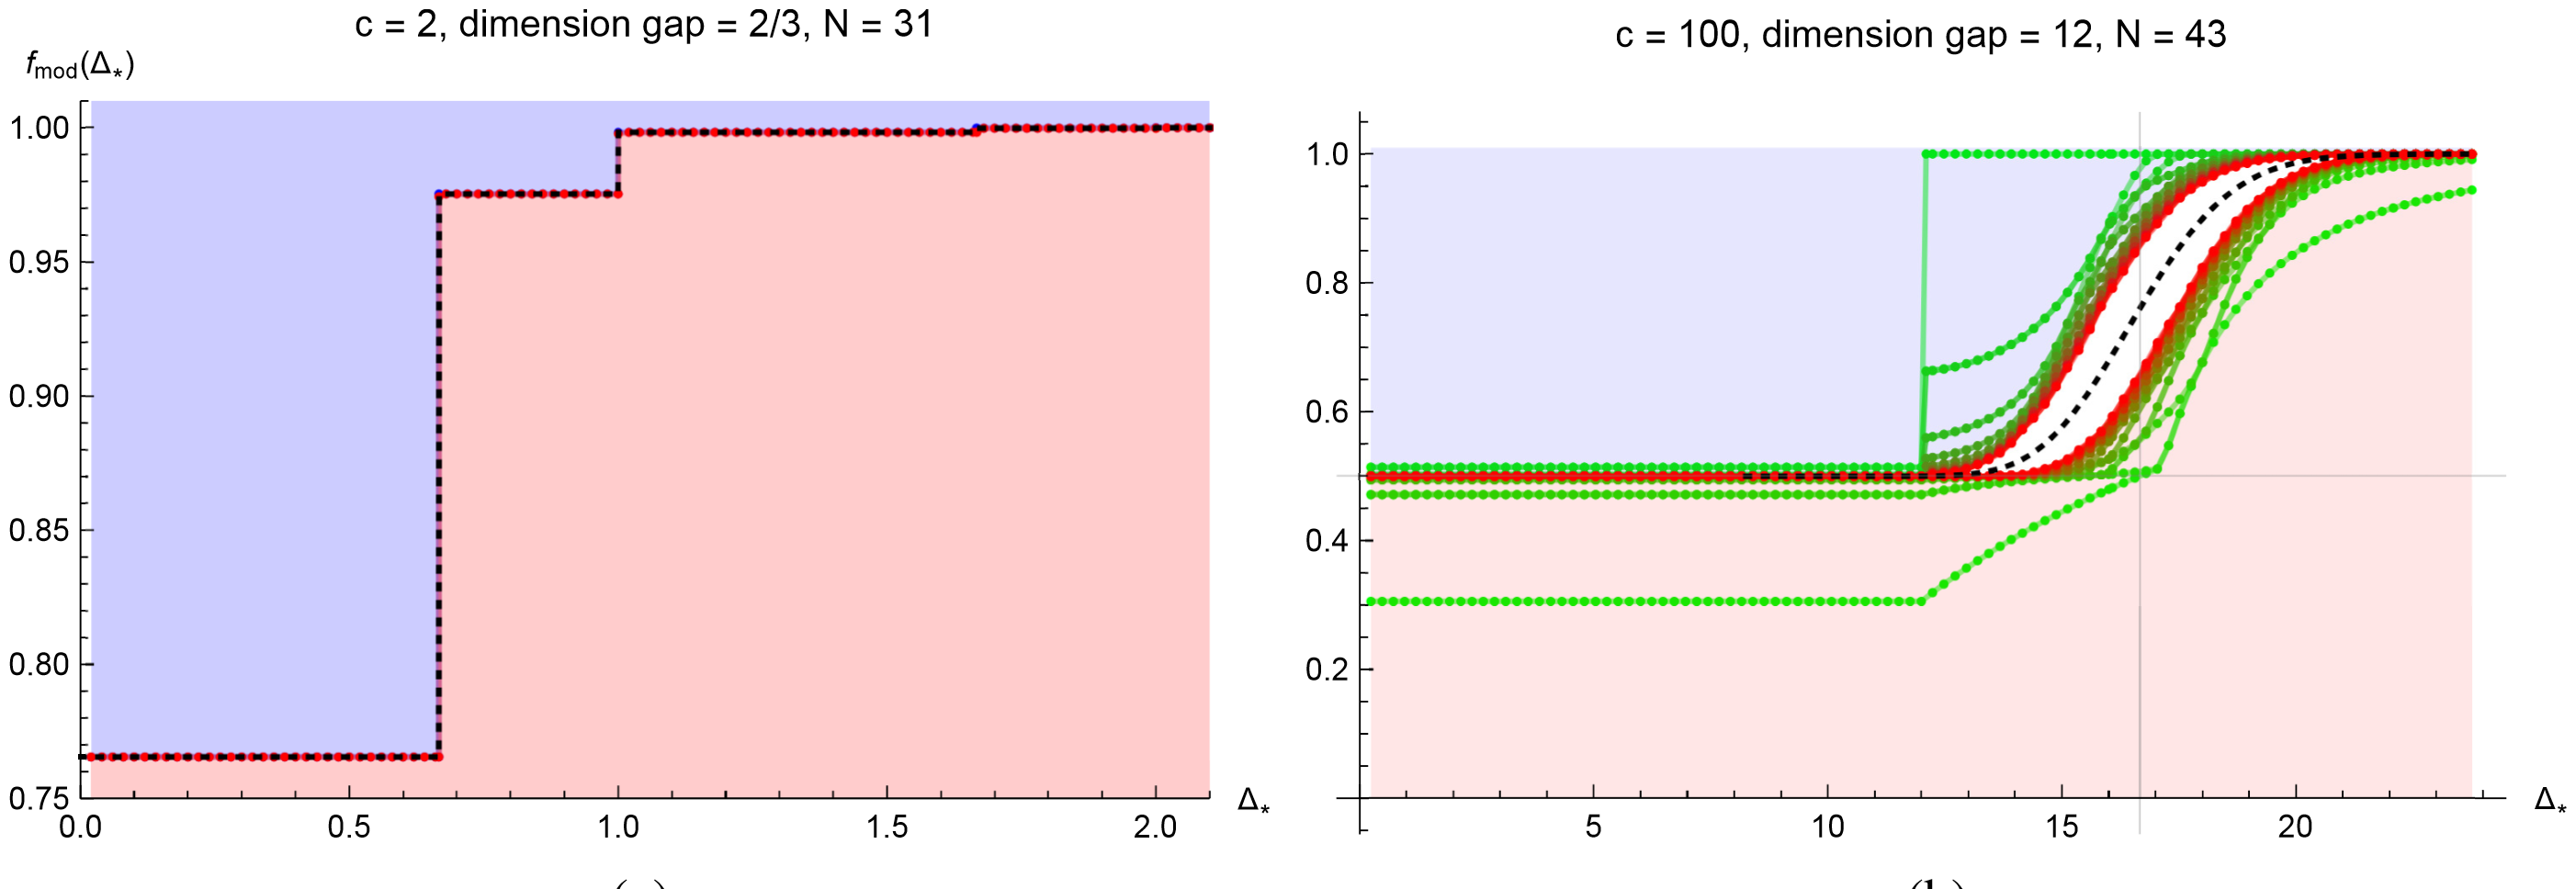
\includegraphics[width=0.85\textwidth]{figures/fig17.png}
  \caption{(a) $c=2$ 时模谱函数的上界（蓝）与下界（红），设间隙等于 $\Delta_{\mathrm{mod}}=\frac23$。(b) $c=100$ 时模谱函数的上、下界，设间隙接近 $\Delta_{\mathrm{mod}}$。黑色虚线是微扰 AdS$_3$ 纯引力的模谱函数，由引力路径积分中的热 AdS$_3$ 鞍点与欧氏 BTZ 鞍点算出。图取自~\cite{r61}。（原文 p.40，图 17）}
  \label{fig:17}
\end{figure}

% [Tutor Note: (5.24) 的分母取 $\tau=-\bar\tau=i$，即 $\tau=i$、$\bar\tau=-i$；$\bar\tau$ 是 $\tau$ 的复共轭，模不变配分函数在自对偶点 $\tau=i$ 的取值正是这样写的，切勿把分母误写成 $Z(\tau=\bar\tau=i)$。]

类似地，我们可以定义模谱函数
\begin{equation}
  \label{eq:5-24}
  f_{\mathrm{mod}}(\Delta_*)
  = \frac{\sum_{h+\tilde h<\Delta_*}\,
      d_{h,\tilde h}\,\chi_h(\tau=i)\,
      \overline{\chi}_{\tilde h}(\bar\tau=-i)}
    {Z(\tau=-\bar\tau=i)},
\end{equation}
并借助模交叉方程、在谱 $\mathcal{S}$ 上作适当假设（比如存在维数间隙 $\Delta_0$）来给它定界。若取 $\Delta_0$ 为维数间隙的模界 $\Delta_{\mathrm{mod}}(c)$，则可期望 $f_{\mathrm{mod}}(\Delta_*)$ 的上、下界收敛并确定谱。实际操作中，用最多 $N$ 阶 $\tau,\bar\tau$ 导数得到的界 $f_{\mathrm{mod},\pm}^{(N)}(\Delta_*)$，在大 $c$ 下随 $N$ 收敛得较慢。

图~\ref{fig:17} 给出模谱函数数值界的两个例子。$c=2$ 时，取最大间隙 $\Delta_{\mathrm{gap}}=\frac23$，界把谱函数确定为 $SU(3)_1$ WZW 模型的谱函数；$c=100$ 时，取接近 $\Delta_{\mathrm{mod}}$ 的间隙，数值界缓慢收敛到 AdS$_3$ 半经典纯引力所预期的答案。

% ===== 原书 p.41（PDF 42）：5.3 节 =====

\subsection{超共形理论的一些结果}\label{sec:5-3}

我们将用两个非平凡的例子，简要介绍超共形场论（SCFT）中关于 BPS 算符 OPE 间隙定界的一些结果。

首先考虑由 K3 上的超对称非线性 sigma 模型定义的 $c=6$ 的 $(4,4)$ SCFT。算符谱可以按小 $\mathcal{N}=4$ 超共形代数（SCA）的表示来组织。在 NS 扇区，表示由超共形原初的权 $h$ 与 $SU(2)_R$ 自旋 $\ell$ 标记。非 BPS 表示 $[h,\ell]$ 满足 $h>\ell$，而 $c=6$ 的 $\mathcal{N}=4$ SCA 中 $SU(2)$ 自旋的允许值只有 $\ell=0$。BPS 表示则满足 $h=\ell$，$\ell$ 可取 $0$ 或 $\frac12$；我们直接把该表示记为 $\langle\ell\rangle$。把手征扇区与反手征扇区合并，得到以下几类表示：
\begin{equation}
  \label{eq:5-25}
  \begin{aligned}
    &\text{vacuum}: \langle 0;0\rangle,\\
    &\tfrac12\text{-BPS}: \langle \tfrac12;\tfrac12\rangle,\\
    &\tfrac14\text{-BPS}: [s,0;\tfrac12\rangle,\
      \langle \tfrac12;s,0],\quad s=1,2,\cdots,\\
    &\text{non-BPS}: [h,0;\tilde h,0],\quad
      h,\tilde h>0,\ h-\tilde h\in\mathbb{Z}.
  \end{aligned}
\end{equation}
% [Tutor Note: (5.25) 用 $(4,4)$ SCA 的表示论组织谱，关键在于 BPS 条件 $h=\ell$：$c=6$ 的小 $\mathcal{N}=4$ 代数中 $SU(2)_R$ 自旋只允许 $0,\frac12$ 的 BPS 值，因此 BPS 原初只分 $\frac12$-BPS 与 $\frac14$-BPS 两类；整理 (5.25) 时勿把 R 自旋 $\ell$ 与共形权 $h$ 混同。]

这里假定工作在共形流形上的一个一般点，即除超共形代数外没有额外守恒流。注意 $\frac14$-BPS 原初有半整数自旋，但其半整数能级的 $\mathcal{N}=4$ 后代自旋为整数，会存活过 GSO 投影。$\frac12$-BPS 与 $\frac14$-BPS 原初的简并度由椭圆亏格决定。结果可总结为如下 BPS 算符内容
\begin{equation}
  \label{eq:5-26}
  \langle 0;0\rangle\oplus 20\langle\tfrac12;\tfrac12\rangle
  \oplus\bigoplus_{s=1}^{\infty} n_s
  \Bigl([s,0;\tfrac12\rangle\oplus\langle\tfrac12;s,0]\Bigr),
\end{equation}
其中 $n_1=90$、$n_2=462$、$n_3=1540$，等等。$20$ 个 $\frac12$-BPS 表示给出 $80$ 个保持 $(4,4)$ SCA 的精确边缘形变，它们对应共形流形
\[
  \mathcal{M}\simeq
  \mathrm{Aut}(\Gamma_{20,4})\backslash SO(20,4)/
  \bigl(SO(20)\times SO(4)\bigr)
\]
的切方向。

% [Tutor Note: $20$ 个 $\frac12$-BPS 表示给出 $80=20\times4$ 个精确边缘形变，而陪集 $\mathrm{Aut}(\Gamma_{20,4})\backslash SO(20,4)/(SO(20)\times SO(4))$ 在一般点的切空间维数正是 $20\times4=80$；这个计数是检验“边缘形变数目”与“模空间维数”是否一致的快速办法。]

尽管 BPS 算符谱沿共形流形 $\mathcal{M}$ 不变（例外是某些特殊点：那里有些非 BPS 原初变成 BPS，并给出额外的守恒高自旋流），非 BPS 算符谱却对精确边缘形变有高度非平凡的依赖。共形流形 $\mathcal{M}$ 可等价地描述为嵌入 $\mathbb{R}^{20,4}$ 的 Narain 格 $\Gamma_{20,4}$ 的模空间。格矢量 $\ell\in\Gamma_{20,4}$ 可按其在 $\mathbb{R}^{20,4}$ 正、负子空间上的投影分解，记为 $(\ell_L,\ell_R)$。只要格的嵌入使某个满足 $\ell^2\equiv\ell_L^2-\ell_R^2=2$ 的格矢量落在正子空间内，即 $\ell_R=0$，模空间中的对应点就给出奇异的 K3 CFT：该 CFT 在某个维数间隙之上发展出连续谱。这类奇点有 ADE 分类，与 IIA 型弦论紧化在 K3 上时六维规范对称性的增强有关。

抓住 K3 CFT 模依赖的一个精确结果如下~\cite{r62,r63}。设 $\phi_i^{\pm,\pm}$ 是 $\frac12$-BPS 的 (NS,NS) 原初，它们在手征与反手征 $SU(2)$ R 对称性的二重态中变换。经半单位谱流，它联系到 (R,R) 原初 $\phi_i^{RR}$，

% ===== 原书 p.42（PDF 43）=====

后者是 R 对称性的单态，共形权为 $(\frac14,\frac14)$。现在考虑积分四点函数
\begin{equation}
  \label{eq:5-27}
  \begin{aligned}
    &\int d^2z\,|z|^{-s-1}|1-z|^{-t-1}
    \bigl\langle \phi_i^{RR}(0)\phi_i^{RR}(z,\bar z)
      \phi_k^{RR}(1)\phi_\ell^{RR'}(\infty)\bigr\rangle\\
    &\quad = 2\pi\left(
      \frac{\delta_{ij}\delta_{k\ell}}{s}
      + \frac{\delta_{i\ell}\delta_{ij}}{t}
      + \frac{\delta_{ik}\delta_{j\ell}}{u}\right)
      + A_{ijk\ell} + B_{ij,k\ell}\,s
      + B_{i\ell,kj}\,t + B_{ik,j\ell}\,u
      + O(s^2,t^2,u^2),
  \end{aligned}
\end{equation}
其中 $u\equiv -s-t$，左端由 $s,t$ 的适当区域解析延拓定义（在该区域积分收敛）；也可以从 $z$ 的被积函数中减去适当的抵消项，直接在 $s=t=0$ 附近展开积分。在 IIB 型弦论紧化于 K3 的语境中，\eqref{eq:5-27} 可解释为六维四个张量多重态的弦树图级散射振幅。利用超对称性，由六维 $(2,0)$ 超引力的超振幅分析得到的非重整化结果（此处不回顾），可以把系数 $A_{ijk\ell}$ 与 $B_{ij,k\ell}$ 确定为 K3 CFT 共形流形上的精确函数。

% [Tutor Note: 原文 (5.27) 有两处疑似笔误：左端第二个算符写作 $\phi_i^{RR}$，按右端系数 $A_{ijk\ell}$、$B_{ij,k\ell}$ 的指标结构应为 $\phi_j^{RR}$；$t$ 道交叉项的分子写作 $\delta_{i\ell}\delta_{ij}$，按 $s,t,u$ 三道的置换对称性应为 $\delta_{i\ell}\delta_{jk}$。译文照原文排，以便与底本逐符号对照。]

% [Tutor Note: 原文在四点函数的第四个算符上一律加撇（本式为 $\phi_\ell^{RR'}$，后文 (5.31) 为 $\phi_1^{RR'}$、(5.32) 为 $\phi^{-,-'}$、(5.44) 为 $\bar\sigma_3'$），而正文叙述中同一算符不带撇；疑为原文排版或记号习惯，译文保留原样。]

例如 $A_{ijk\ell}$ 由
\begin{equation}
  \label{eq:5-28}
  A_{ijk\ell}
  = \frac{1}{16\pi^2}\,
    \frac{\partial^4}{\partial y^i\partial y^j\partial y^k\partial y^\ell}
    \bigg|_{y=0}
    \int_{\mathcal{F}} d^2\tau\,
    \frac{\Theta_\Lambda(y|\tau,\bar\tau)}{(\eta(\tau))^{24}},
\end{equation}
给出，其中 $\mathcal{F}$ 是 $PSL(2,\mathbb{Z})$ 作用在上半平面上的基本区域，$\Lambda$ 表示嵌入 $\mathbb{R}^{20,4}$ 的格 $\Gamma_{20,4}$，它参数化 K3 CFT 共形流形上的一点。格 theta 函数 $\Theta_\Lambda$ 定义为
\begin{equation}
  \label{eq:5-29}
  \Theta_\Lambda(y|\tau,\bar\tau)
  = e^{\frac{\pi}{2\tau_2}y^2}
    \sum_{\ell\in\Lambda}
    e^{i\pi\tau\ell_L^2 - i\pi\bar\tau\ell_R^2
      + 2\pi i\,\ell_L\cdot y}.
\end{equation}
辅助矢量 $y$ 位于正子空间 $\mathbb{R}^{20}$，其分量与 K3 CFT 的 $20$ 个 $\frac12$-BPS 多重态对应。公式~\eqref{eq:5-28} 可从杂化弦/II 型对偶理解为杂化弦单圈振幅，因此要对环面的模积分。$B_{ij,k\ell}$ 有类似的公式，是对亏格二黎曼面模的积分。

% [Tutor Note: (5.29) 中 $\ell_L^2$ 与 $\ell_R^2$ 的系数分别是 $+i\pi\tau$ 与 $-i\pi\bar\tau$，$\bar\tau$ 前的负号最易漏；归一化因子里的 $\tau_2$ 指 $\mathrm{Im}\,\tau$，不要写成 $\bar\tau$。]

% [Tutor Note: (5.28) 的四阶导数在 $y=0$ 取值，而 $y$ 只跑正子空间 $\mathbb{R}^{20}$ 的 $20$ 个分量；$\Theta_\Lambda$ 对 $y$ 的依赖为 $e^{\frac{\pi}{2\tau_2}y^2+2\pi i\ell_L\cdot y}$，逐次求导时高斯因子同样贡献项，不要只对 $e^{2\pi i\ell_L\cdot y}$ 求导。]

我们只用单个原初（比如 $\phi_1^{RR}$）的积分四点函数，即 $A_{1111}$。结果 $A_{1111}$ 取非负实值，并在两种不同极限下发散：(1) 满足 $\ell^2=2$ 的格矢量落在正子空间内，对应 K3 出现 $A_1$ 奇点；或 (2) 零格矢量（即 $\ell_L^2=\ell_R^2$）有 $\ell_L^2,\ell_R^2\to0$，对应 K3 曲面的大体积极限。我们希望把 $\phi_1^{RR}\phi_1^{RR}$ OPE 的非 BPS 算符内容约束为 $A_{1111}$ 的函数，后者编码了对共形流形的依赖~\cite{r64}。

为继续，需要把 $\frac12$-BPS 四点函数按 $(4,4)$ SCA 的超 Virasoro 共形块分解。对 Ward 恒等式作简单分析即可看出：一对 $\frac12$-BPS 原初的 OPE 中可能出现的表示，只有真空/单位表示与非 BPS 表示（后者的 $SU(2)_R$ 自旋必为零）。

% ===== 原书 p.43（PDF 44）=====

BPS 关联子 $\langle\phi^R(0)\phi^R(z)\phi^R(1)\phi^{R'}(\infty)\rangle$（外部算符为 R 扇区中权 $\frac14$ 的算符）在标号为 $[h,0]$ 的非 BPS 道中的手征 $c=6$ $\mathcal{N}=4$ 超共形块，等于外权为 $1$、内权为 $h+1$ 的 $c=28$ 玻色 Virasoro 块，二者只相差一个简单的前因子：
\begin{equation}
  \label{eq:5-30}
  \mathcal{F}_h^{\mathcal{N}=4,R}(z)
  = z^{\frac12}(1-z)^{\frac12}\,
    \mathcal{F}_{c=28}^{\text{Virasoro}}(1,1,1,1,h+1;z).
\end{equation}
这个简单关系成立的原因是：(1) $c=6$ 的 $\mathcal{N}=4$ 超共形块恰好与 $\mathcal{N}=2$ 子代数的对应块重合（$c\ge 12$ 时并非如此）；(2) 含外部 BPS 算符的 $\mathcal{N}=2$ 块与 Virasoro 共形块以简单方式相联系，这可以通过研究 $\mathcal{N}=2$ cigar CFT 的关联子来论证。真空道块可由~\eqref{eq:5-30} 的 $h\to0$ 极限得到。

% [Tutor Note: 注意 (5.30) 的玻色块内权是 $h+1$：$h$ 是 $\mathcal{N}=4$ 超共形权，并非 $c=28$ Virasoro 块的内权；真空道（$h\to0$）对应的是内权为 $1$ 的玻色块，勿直接把内权也取成 $h$。]

\begin{figure}[htbp]
  \centering
  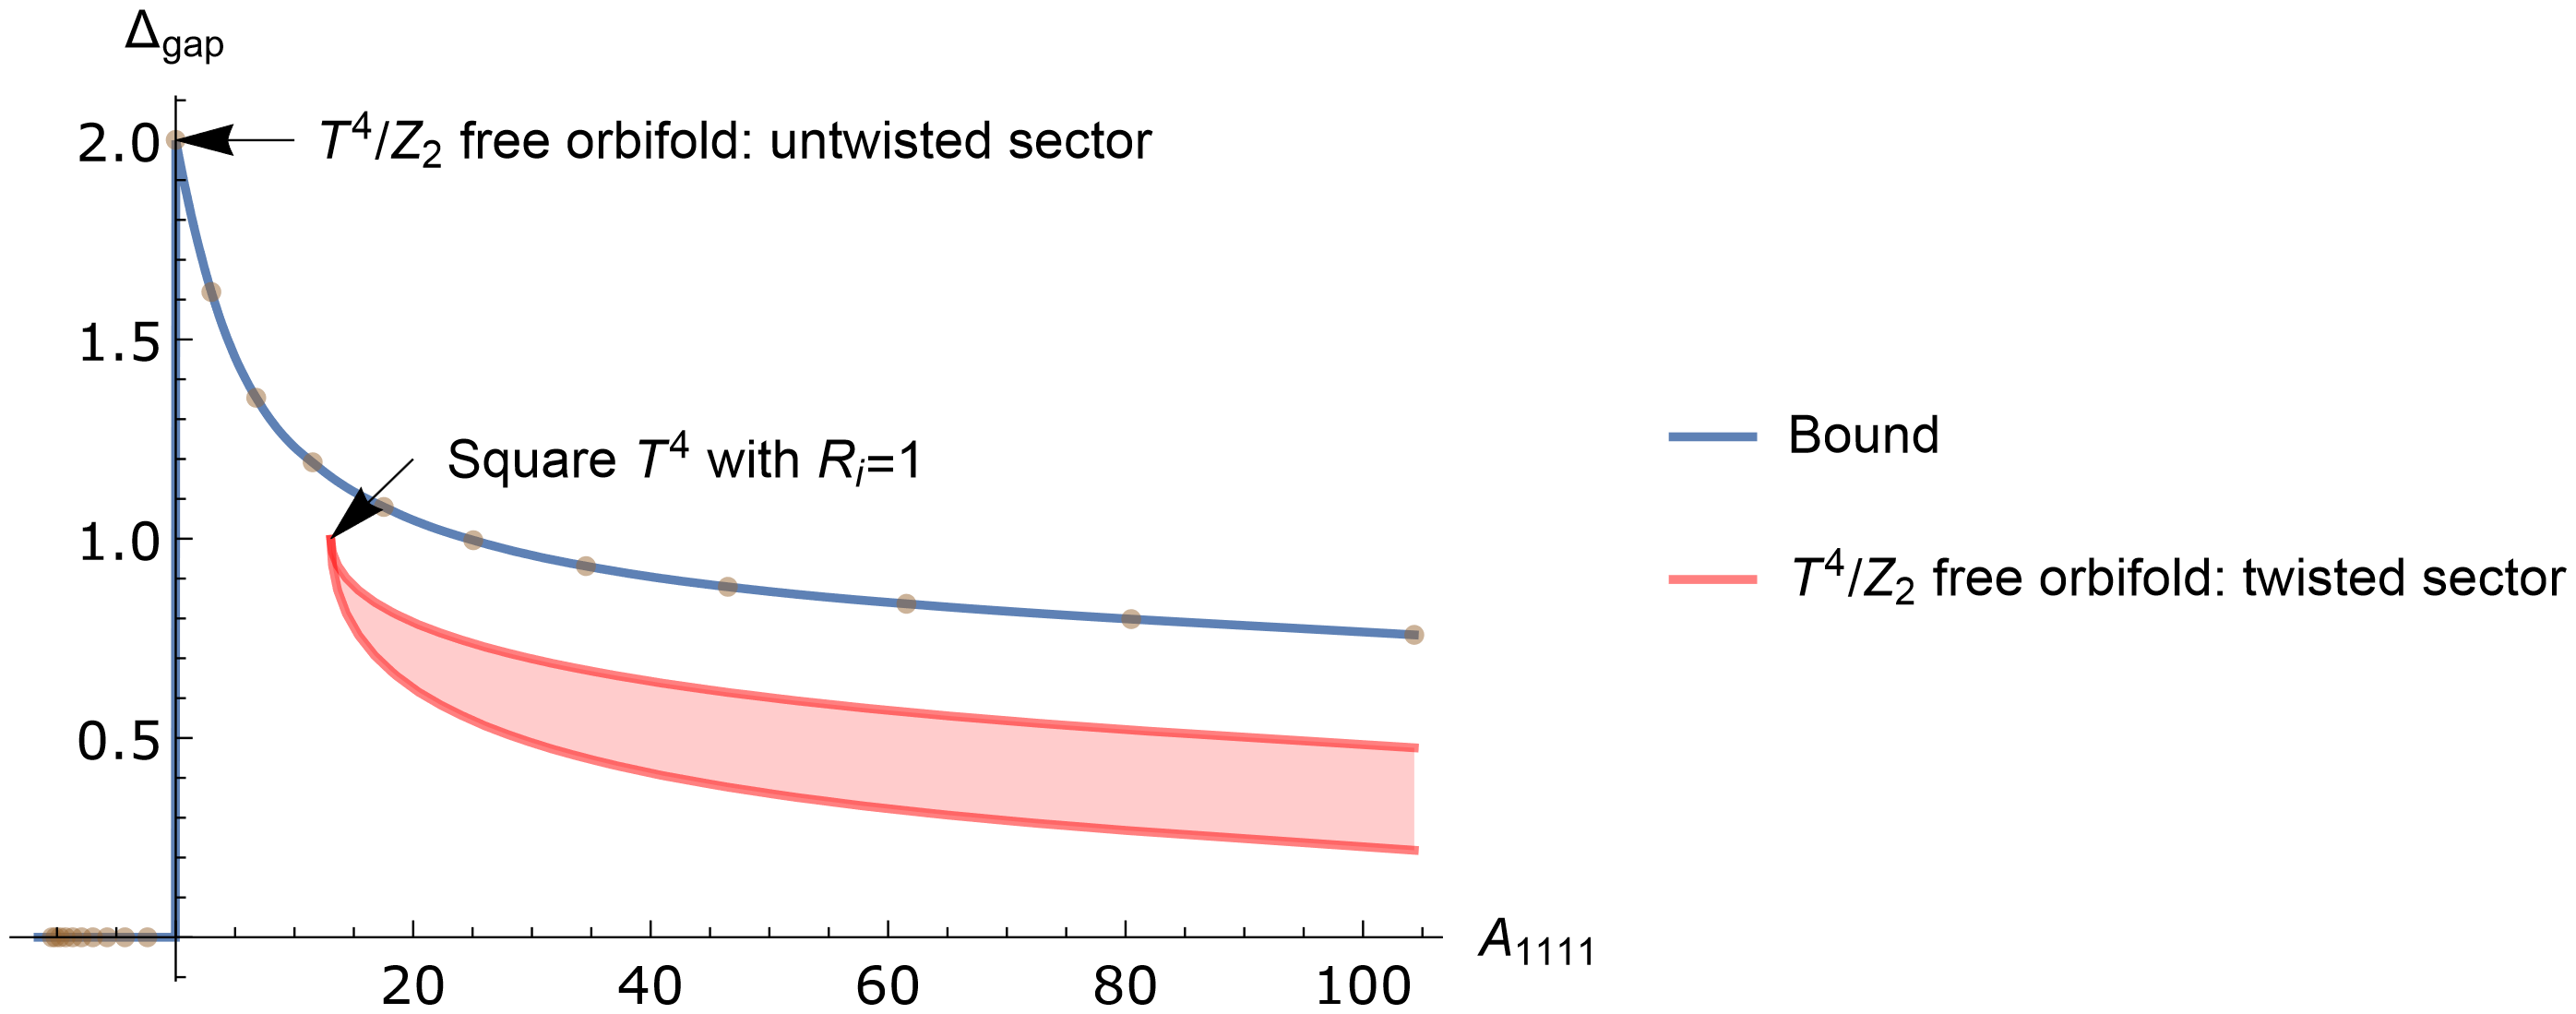
\includegraphics[width=0.85\textwidth]{figures/fig18.png}
  \caption{实心蓝线给出 $\phi_1\phi_1$ OPE 中非 BPS 原初间隙的上界，横轴是积分 BPS 四点函数 $A_{1111}$（橙色圆点是数值数据点，它们在 $20$ 阶导数处已经稳定）。红色阴影区域表示 $T^4/\mathbb{Z}_2$ 某个不动点处 $\frac12$-BPS 扭曲场 OPE 中的间隙，该不动点处 $T^4$ 为矩形。图取自~\cite{r64}。（原文 p.43，图 18）}
  \label{fig:18}
\end{figure}

现在，我们直接对关联子
\begin{equation}
  \label{eq:5-31}
  \bigl\langle \phi_1^{RR}(0)\phi_1^{RR}(z,\bar z)
    \phi_1^{RR}(1)\phi_1^{RR'}(\infty)\bigr\rangle
  = \sum_{h,\tilde h} C_{h,\tilde h}^2\,
    \mathcal{F}_h^{\mathcal{N}=4,R}(z)\,
    \overline{\mathcal{F}}_{h}^{\mathcal{N}=4,R}(\bar z).
\end{equation}
% [Tutor Note: (5.31) 右端第二个块的下标，原文印刷为不带波浪的 $h$（与求和的 $h,\tilde h$ 不一致），译文照原样保留。此处按右移权记作 $\tilde h$ 才是通常的分解，属原文疑似笔误。]
施加交叉方程的约束。来自 $A_{1111}$ 的约束可简单地表述为对 $C_{h,\tilde h}^2$ 的一条额外线性关系，它与交叉方程处于同等地位。分析细节太长，此处不再复述；我们直接把 $\phi_1\phi_1$ OPE 中第一个非 BPS 原初维数间隙上界的结果总结在图~\ref{fig:18} 中。

% [Tutor Note: (5.31) 把交叉方程写成正系数 $C_{h,\tilde h}^2$ 的线性组合，这正是能化为半正定规划的标准形式；对照后面 (5.33) 的结构常数 $C_{ijj}$ 没有先验正性，环面一点函数的模协变约束便难以直接用同一数值方法处理，这是作者在 5.4 节转向亏格二配分函数的动机之一。]

在 $A_{1111}\to\infty$ 极限下，维数间隙界的渐近值从图~\ref{fig:18} 的绘图范围看不出，但数值上求得为 $\Delta_{\mathrm{gap}}=\frac14$。这个值实际上被 $\mathcal{N}=4$ 的 $A_1$ cigar CFT 饱和；该理论有精确描述，即超对称的 $SL(2,\mathbb{R})_2/U(1)$ 陪集，并被猜想能刻画 K3 CFT 出现 $A_1$ 奇点时的奇异极限。

另一个例子我们只作极简讨论：$c=9$ 的 $(2,2)$ SCFT 中 $\frac12$-BPS 算符 OPE 内容的约束~\cite{r65}。这类理论包括 Calabi--Yau 三维流形上的超对称非线性 sigma 模型。如前所述，后者有扩充的 $\mathcal{N}=2$ SCA，这对 BPS 算符的三点函数给出高度非平凡的约束。

% ===== 原书 p.44（PDF 45）=====

在某些情形，比如五次三维流形上的 NLSM，诸如 (chiral, chiral) $\frac12$-BPS 算符的三点函数已被确定为共形流形上的精确函数。这使我们能通过 BPS 算符的 OPE 系数，把模依赖纳入 $\frac12$-BPS 四点函数的分析，从而用交叉方程约束 OPE 的非 BPS 算符内容。

令 $\phi^{+,+}$ 是权为 $(\frac12,\frac12)$ 的 (chiral, chiral) 原初，$\phi^{-,-}$ 是其共轭的 (anti-chiral, anti-chiral) 原初。我们可以按 $\phi^{+,+}\phi^{+,+}$ OPE 道（CC）与 $\phi^{+,+}\phi^{-,-}$ OPE 道（CA）中的 $\mathcal{N}=2$ 超共形块分解来分析四点函数
\begin{equation}
  \label{eq:5-32}
  \bigl\langle \phi^{+,+}(0)\phi^{-,-}(z,\bar z)
    \phi^{+,+}(1)\phi^{-,-'}(\infty)\bigr\rangle,
\end{equation}
并利用 $z\to1-z$ 交叉方程同时约束两个道中第一个非 BPS 原初的间隙。

模依赖可通过 $\phi^{+,+}\phi^{+,+}$ OPE 中一个 R 荷为 $(2,2)$ 的 BPS 原初的 OPE 系数 $\lambda$ 纳入。图~\ref{fig:19} 给出 CC 对 CA 道中非 BPS 谱间隙数值界随 $\lambda$ 变化的一个例子，施用于五次三维流形模型；其中 $\phi^{+,+}$ 是与 Kähler 形变相联系的 BPS 原初，BPS OPE 系数 $\lambda$ 是 Kähler 模空间上的已知函数。可以看到，边界曲面上有些点由自由理论的 OPE 饱和。

\begin{figure}[htbp]
  \centering
  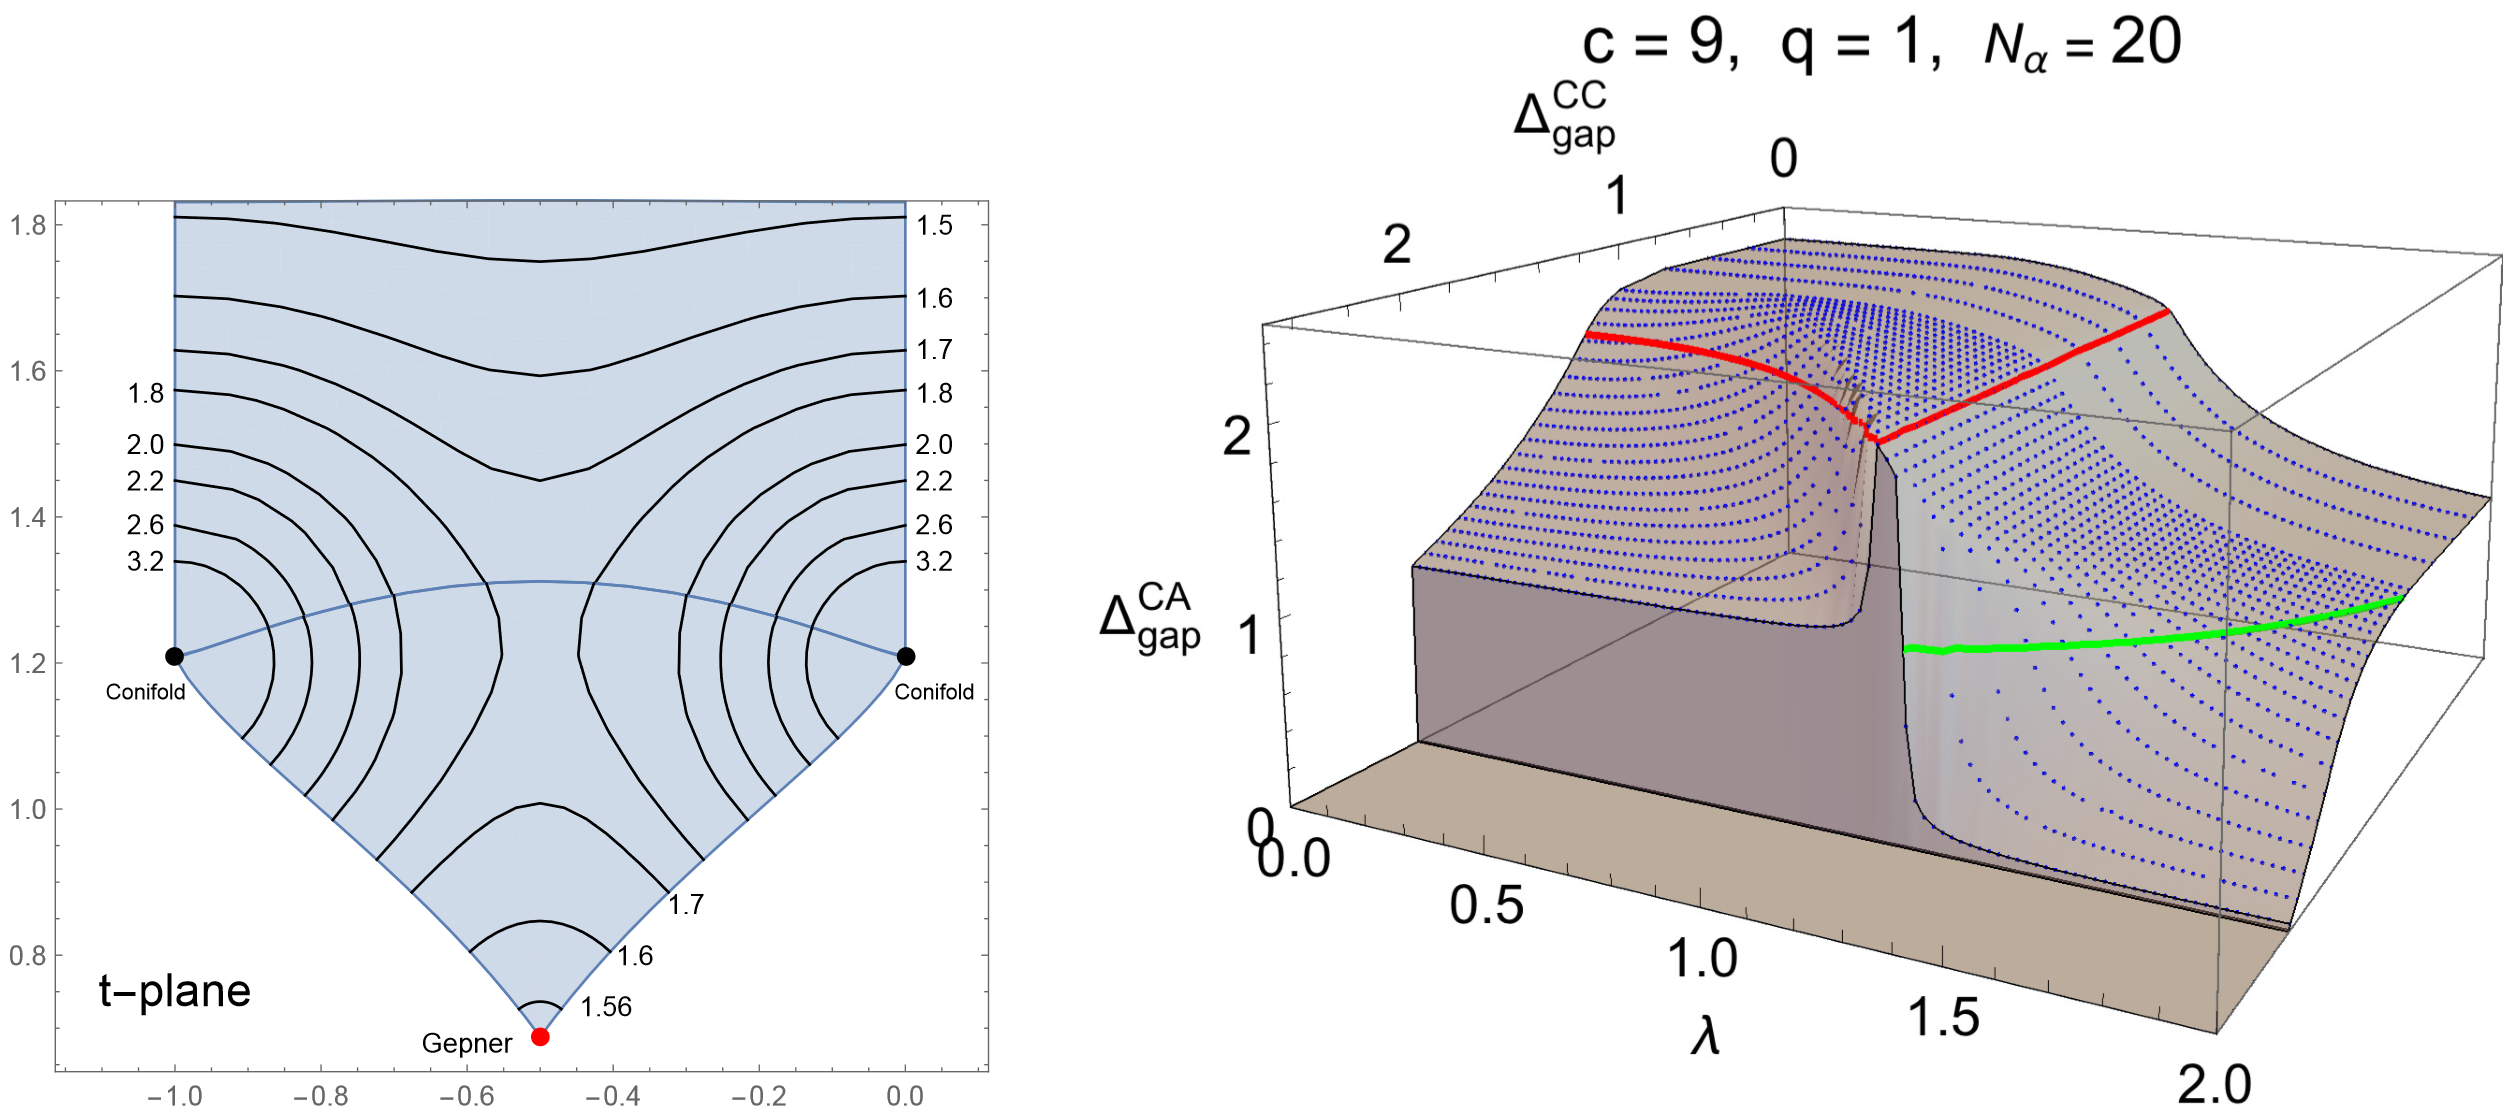
\includegraphics[width=0.85\textwidth]{figures/fig19.png}
  \caption{左：五次三维流形 Kähler 模空间上手征环系数 $\lambda$ 的等值线图~\cite{r66}。黑曲线是 $\lambda$ 的等值线；conifold 点用黑点标出，Gepner 点用红色标出。右：CA 道中间隙 $\Delta_{\mathrm{gap}}^{CA}$ 作为 $\Delta_{\mathrm{gap}}^{CC}$ 与 $\lambda$ 的函数的上界，用最多 $20$ 阶导数的线性泛函算出。$\Delta_{\mathrm{gap}}^{CC}=2$ 截面上的窄峰，预计在导数阶数趋于无穷时收缩为零宽度。图取自~\cite{r65}。（原文 p.44，图 19）}
  \label{fig:19}
\end{figure}

% [Tutor Note: CC 道指 $\phi^{+,+}\phi^{+,+}$ OPE，CA 道指 $\phi^{+,+}\phi^{-,-}$ OPE；$z\to1-z$ 交叉方程把两个道的间隙联系起来。图 19 右图的边界曲面同时约束两个道的间隙，纵轴是 $\Delta^{CA}_{\mathrm{gap}}$，不要把 $\Delta^{CC}_{\mathrm{gap}}$ 也当成纵轴。]

% ===== 原书 p.44 末（PDF 45）：5.4 节开始 =====

\subsection{亏格二模自举}\label{sec:5-4}

到目前为止，我们分析了交叉对称性对单个 OPE 的约束，以及配分函数的模不变性对谱的约束。可以把后者推广到环面一点函数的模协变性。

% ===== 原书 p.45（PDF 46）=====

事实上，把原初 $\phi_i(z,\bar z)$ 的环面一点函数按环面一点 Virasoro 共形块分解，
\begin{equation}
  \label{eq:5-33}
  \bigl\langle \phi_i(z,\bar z)\bigr\rangle_{T^2(\tau)}
  = \sum_j C_{ijj}\,
    \mathcal{F}_c^{T^2}(h_i,h_j,h_j;\tau)\,
    \overline{\mathcal{F}}_c^{T^2}
      (\tilde h_i,\tilde h_j,\tilde h_j;\bar\tau),
\end{equation}
就很容易把关于 $\tau\to-1/\tau$ 的模交叉方程写成一族关于结构常数 $C_{ijj}$ 的线性关系。然而 $C_{ijj}$ 没有先验的正性，用半正定规划实现这类约束并不容易。

至于球面四点函数的交叉方程，最终我们希望同时合并 CFT 中所有原初的交叉方程，但除少数几个原初外这非常困难。因此，球面四点交叉方程与环面一点函数的模协变性原则上给出了二维幺正 CFT 的完整相容关系集。但我们仍需要以某种方式组织这些交叉方程，使其计入大量原初的 OPE，并满足一定的正性。

考虑 CFT 在亏格二黎曼面上配分函数的模约束，可以部分做到这一点。这样的配分函数可分解为亏格二 Virasoro 共形块，其系数涉及 $C_{ijk}^2$ 或 $C_{ijj}C_{ikk}$。这里只关注前者。亏格二黎曼面的模空间复维数为 $3$，可用多种方式参数化。下面描述三种参数化。

第一种参数化通过周期矩阵
\begin{equation}
  \label{eq:5-34}
  \Omega = \begin{pmatrix}
    \Omega_{11} & \Omega_{12}\\
    \Omega_{21} & \Omega_{22}
  \end{pmatrix},
\end{equation}
它满足 $\Omega^T=\Omega$ 且 $\mathrm{Im}\,\Omega$ 正定。元素 $\Omega_{ab}$ 定义如下。取一维同调群 $H_1(\Sigma_2,\mathbb{Z})$ 的一组基 $\alpha_1,\alpha_2,\beta_1,\beta_2$，相交数 $\alpha_a\cdot\alpha_b=\beta_a\cdot\beta_b=0$、$\alpha_a\cdot\beta_b=\delta_{ab}$。存在两个独立的全纯 1-形式 $\omega_a$，$a=1,2$，使得
\begin{equation}
  \label{eq:5-35}
  \oint_{\alpha_a}\omega_b = \delta_{ab},
  \qquad
  \oint_{\beta_a}\omega_b = \Omega_{ab}.
\end{equation}
基 $\{\alpha_a,\beta_a\}$ 在 $Sp(4,\mathbb{Z})$ 变换下定义到形如
\begin{equation}
  \label{eq:5-36}
  \alpha_a \to D_{ab}\alpha_b + C_{ab}\beta_b,
  \qquad
  \beta_a \to B_{ab}\alpha_b + A_{ab}\beta_b,
\end{equation}
的变换，其中 $2\times2$ 矩阵 $A,B,C,D$ 的元素为整数，并满足
\begin{equation}
  \label{eq:5-37}
  \gamma
  \begin{pmatrix}
    0 & \mathbb{I}\\
    -\mathbb{I} & 0
  \end{pmatrix}
  \gamma^T
  =
  \begin{pmatrix}
    0 & \mathbb{I}\\
    -\mathbb{I} & 0
  \end{pmatrix},
  \qquad
  \gamma\equiv
  \begin{pmatrix}
    A & B\\
    C & D
  \end{pmatrix}.
\end{equation}
相应地，周期矩阵按
\begin{equation}
  \label{eq:5-38}
  \Omega \mapsto \gamma(\Omega)
  \equiv (A\Omega+B)(C\Omega+D)^{-1}
\end{equation}
变换。

% [Tutor Note: (5.35) 采用 A-周期归一化为单位矩阵、B-周期给出周期矩阵的约定；不少文献把 B-周期的符号取反，代入 (5.38) 前须核对同一约定，否则 $B,C$ 的符号会整体反号（(5.36) 与 (5.37) 中的 $B,C$ 随之反号）。]

% [Tutor Note: (5.38) 的矩阵乘法次序是 $(A\Omega+B)(C\Omega+D)^{-1}$，一般不可交换，切勿写成 $(C\Omega+D)^{-1}(A\Omega+B)$；这是核对 $Sp(4,\mathbb{Z})$ 作用是否写对的最快检查点。]

% ===== 原书 p.45 末至 p.46（PDF 46--47）=====

CFT 的亏格二配分函数 $Z_2$ 可写成 $(\Omega,\bar\Omega)$ 在 Siegel 上半空间 $\mathrm{Im}\,\Omega\succ0$ 上的函数，并可能在某些 $(\gamma(\Omega))_{12}=0$ 的轨迹上有奇点，其中 $\gamma\in Sp(4,\mathbb{Z})$；除一个只依赖中心荷 $c$ 的普适共形反常因子外，它是良定义的。因此，要指定 $Z_2$ 必须指定一个共形框架，或等价地，在其共形等价类中选定一个度规。稍后我们讨论两个特别有用的共形框架。或者，可以完全避开共形反常，改而考虑比值 $Z_2/(Z_X)^c$，其中 $Z_X$ 是某个给定 $c=1$ CFT（比如自由玻色子）在同一共形框架下的亏格二配分函数。$Z_2/(Z_X)^c$ 便是 $(\Omega,\bar\Omega)$ 的良定义函数，并在~\eqref{eq:5-38} 下不变。

第二种参数化是 Schottky 参数化：把亏格二黎曼面实现为商
\begin{equation}
  \label{eq:5-39}
  \bigl(\mathbb{C}\cup\{\infty\}-\Lambda\bigr)
  \big/\langle\alpha,\beta\rangle,
\end{equation}
其中 $\alpha,\beta$ 是 $PSL(2,\mathbb{C})$ 的两个斜驶元素，$\langle\alpha,\beta\rangle$ 是由 $\alpha$ 与 $\beta$ 生成的自由（非阿贝尔）群，称为 Schottky 群；$\Lambda$ 是 Schottky 群作用的极限集。有一个用 Schottky 群元素上的无穷乘积表示周期矩阵的有用公式，此处不详述。由于它与 AdS$_3$ 引力的联系，Schottky 参数化在写出亏格二（及更高亏格）Virasoro 共形块的经典极限（$c\to\infty$）时很有用。

第三种参数化与 Schottky 参数化密切相关，对计算一般 Virasoro 共形块很有用。它基于管道化构造：把复平面上一对双孔圆盘沿边界粘合，用三个 $PSL(2,\mathbb{C})$ 变换得到亏格二黎曼面。可以取粘合映射为形如 $z\mapsto q/z$ 的反演映射（复参数 $q$，把原点（必要时平移）周围的一对内侧圆周边界等同），或形如 $z\mapsto qz$ 的缩放映射（把一个内侧圆周边界与一个外侧边界等同）。三个复管道参数 $q_i$，$i=1,2,3$，是所得黎曼面的模。

% [Tutor Note: 第三种参数化里的粘合映射是反演 $z\mapsto q/z$ 与缩放 $z\mapsto qz$；三个管道参数 $q_i$ 与 Schottky 参数化中的乘子 $q_\gamma$ 不是同一组变量，对照 (5.40) 与 (5.41) 时注意区分。]

管道化构造也指定了一个共形框架，称为管道框架。管道框架中的 Virasoro 共形块有特殊性质：固定原初权时其 $c\to\infty$ 极限有限，从而允许关于 $c$ 的递推表示，推广了 Zamolodchikov 关于球面四点块的递推公式。一般递推公式示意为
\begin{equation}
  \label{eq:5-40}
  \begin{aligned}
    &\mathcal{G}_c\bigl(\{h_a^{\mathrm{ext}}\};\{h_i\};\{q_i\}\bigr)
    = \mathcal{G}_\infty(0;0;\{q_j\})\,
      \mathcal{G}_{SL(2)}\bigl(\{h_a^{\mathrm{ext}}\};\{h_i\};\{q_i\}\bigr)\\
    &\quad + \sum_j\sum_{r\ge2,\,s\ge1}
      \frac{Q_j^{r,s}}{c-c_{rs}(h_j)}\,
      \mathcal{G}_{c_{rs}(h_j)}
      \bigl(\{h_a^{\mathrm{ext}}\};h_j\to h_j+rs;\{q_i\}\bigr),
  \end{aligned}
\end{equation}
其中 $h_a^{\mathrm{ext}}$ 表示可能的外部权，$h_i$ 是内部权，$q_i$ 是管道参数。$\mathcal{G}_\infty(0;0;\{q_j\})$ 是管道框架中真空块的 $c\to\infty$ 极限，$\mathcal{G}_{SL(2)}$ 是相应的整体 $SL(2,\mathbb{C})$ 共形块。第二行的求和遍历以指标 $j$ 标记的内部权；$Q_j^{r,s}$ 是 $h_j$ 及其在共形块所联系的三价图上相邻权的已知函数。求和项中的 $\mathcal{G}_{c_{rs}(h_j)}$ 是中心荷取 $c_{rs}(h_j)$、内部权 $h_j$ 平移为 $h_j+rs$ 时的共形块。$\mathcal{G}_{SL(2)}$ 可按管道参数展开直接计算。

% ===== 原书 p.47（PDF 48）=====

真空块可用 Schottky 参数化写成闭式~\cite{r67}：
\begin{equation}
  \label{eq:5-41}
  \mathcal{G}_\infty(0;0;\{q_j\})
  = \prod_{\gamma\in\mathcal{P}}\prod_{n=2}^{\infty}
    (1-q_\gamma^n)^{-\frac12},
\end{equation}
其中 $\mathcal{P}$ 是 Schottky 群的本原共轭类的集合。$q_\gamma$ 定义如下：在类 $\gamma$ 中任取一个元素，作为 $PSL(2,\mathbb{C})$ 的元素，它与
\[
  \begin{pmatrix}
    q_\gamma^{1/2} & 0\\
    0 & q_\gamma^{-1/2}
  \end{pmatrix}
\]
共轭，且 $|q_\gamma|<1$。

然而，管道框架中算出的配分函数并不显式模不变，原因在共形反常因子。为以可计算的方式表述模交叉方程，我们改用另一个共形框架，称为 Rényi 框架~\cite{r68}。

\begin{figure}[htbp]
  \centering
  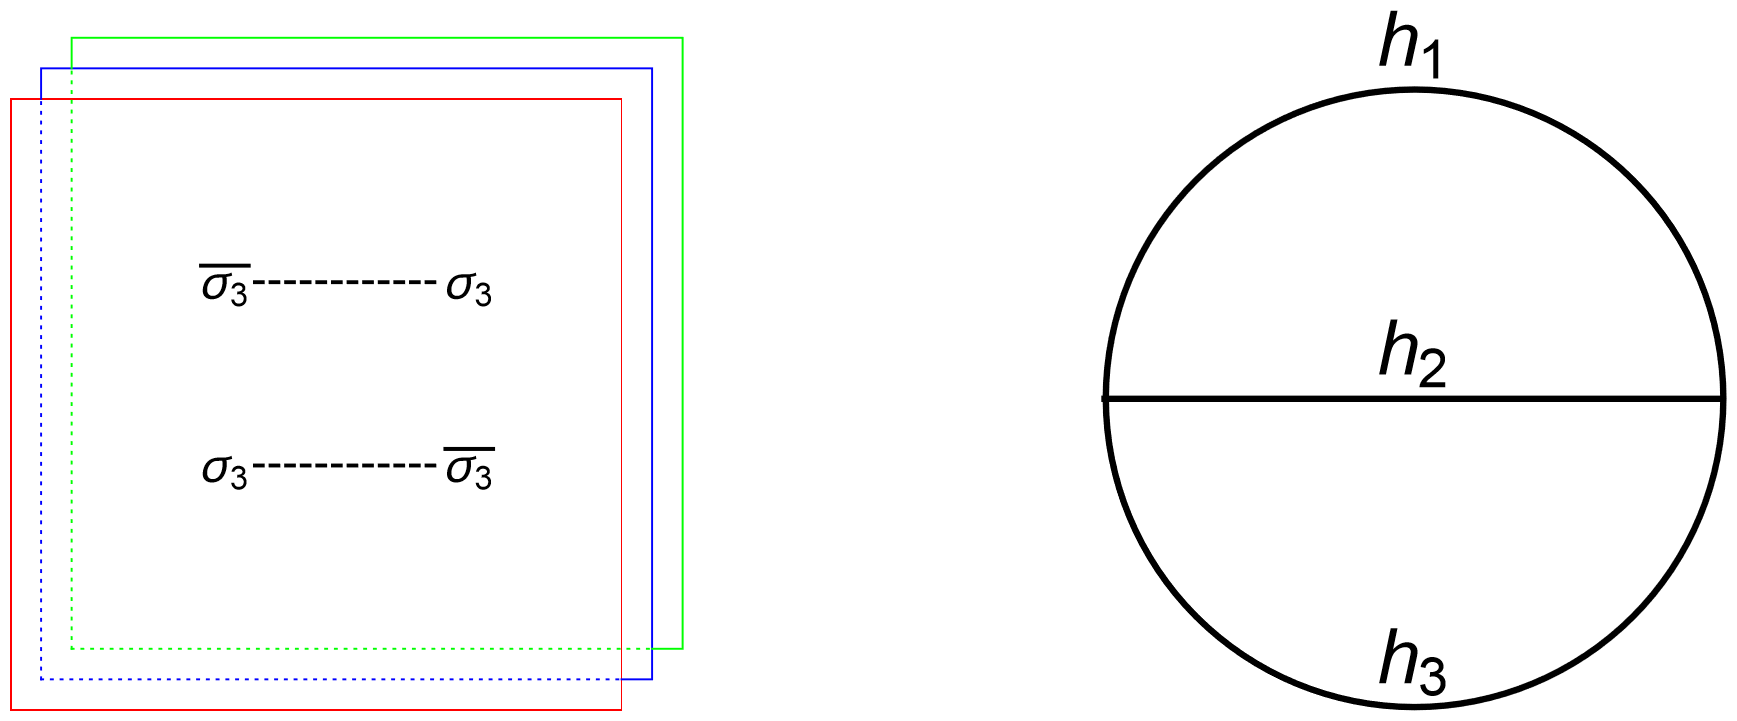
\includegraphics[width=0.85\textwidth]{figures/fig20.png}
  \caption{左：带四个分支点的黎曼球面的三折覆盖是亏格二曲面。覆盖曲面上 CFT 的配分函数可看作球面上三折对称积 CFT 中 $Z_3$ 扭曲场的四点函数。右：与 $\sigma_3\bar\sigma_3$ OPE 道相联系的亏格二共形块。（原文 p.47，图 20）}
  \label{fig:20}
\end{figure}

我们从“Rényi 曲面”出发：它是亏格二黎曼面模空间中的一条复一维轨迹，即黎曼球面在四个分支点处的三折覆盖。明确地说，可把 Rényi 曲面实现为 $\mathbb{CP}^1\times\mathbb{CP}^1$ 中的一条曲线，用仿射坐标 $(x,y)$ 写为
\begin{equation}
  \label{eq:5-42}
  y^3 = \frac{(x-x_1^+)(x-x_2^+)}
             {(x-x_1^-)(x-x_2^-)}.
\end{equation}
在由覆盖映射指定的特定共形框架下，Rényi 曲面上的亏格二配分函数等于黎曼球面上三重对称积 CFT 中一对 $Z_3$ 扭曲场 $\sigma_3$ 与一对反扭曲场 $\bar\sigma_3$ 的四点函数
\begin{equation}
  \label{eq:5-43}
  \bigl\langle \sigma_3(x_1^+)\sigma_3(x_2^+)
    \bar\sigma_3(x_1^-)\bar\sigma_3(x_2^-)\bigr\rangle,
\end{equation}
其亏格二共形块分解为
\begin{equation}
  \label{eq:5-44}
  \bigl\langle \sigma_3(0)\bar\sigma_3(z,\bar z)
    \sigma_3(1)\bar\sigma_3'(\infty)\bigr\rangle
  = \sum_{i,j,k} C_{ijk}^2\,
    \mathcal{F}_c(h_i,h_j,h_k;z)\,
    \overline{\mathcal{F}}_c
      (\tilde h_i,\tilde h_j,\tilde h_k;\bar z),
\end{equation}
其中共形块 $\mathcal{F}_c(h_i,h_j,h_k;z)$ 可通过直接对 $\sigma_3\bar\sigma_3$ OPE 中 Virasoro$^{\otimes 3}$ 后代的贡献求和，按 $z$ 展开计算。Rényi 框架共形块与 Rényi 曲面（仍由同一交比 $z$ 参数化）的管道框架块 $\mathcal{G}_c$ 相差一个共形反常因子：

% [Tutor Note: (5.44) 中的外权是扭曲场的权：对 $Z_3$ 覆盖，$\sigma_3$ 的共形权为 $h_\sigma=\frac{c}{24}(3-\frac13)=\frac{c}{9}$（$Z_2$ 覆盖时为 $\frac{c}{16}$）；代入 (5.47) 时要把 $h_1+h_2+h_3$ 取成 $3h_\sigma$，而不是 $0$。]

% ===== 原书 p.48（PDF 49）=====

\begin{equation}
  \label{eq:5-45}
  \mathcal{F}_c(h_1,h_2,h_3;z)
  = \exp\bigl[c\,\mathcal{F}^{cl}(z)\bigr]\,
    \mathcal{G}_c(h_1,h_2,h_3;z).
\end{equation}
这里记下 $\mathcal{F}^{cl}$ 的 $z$-展开前几项：
\begin{equation}
  \label{eq:5-46}
  \begin{aligned}
    \mathcal{F}^{cl}(z)
    = {}& -\frac{2}{9}\log(z)
      + 6\left(\frac{z}{27}\right)^2
      + 162\left(\frac{z}{27}\right)^3
      + 3975\left(\frac{z}{27}\right)^4\\
      & + 96552\left(\frac{z}{27}\right)^5
      + 2356039\left(\frac{z}{27}\right)^6
      + \cdots,
  \end{aligned}
\end{equation}
以及一般权 $h_1,h_2,h_3$ 下 $\mathcal{G}_c$ 的 $c\to\infty$ 极限：
\begin{equation}
  \label{eq:5-47}
  \begin{aligned}
    &\mathcal{G}_\infty(h_1,h_2,h_3;z)\\
    &\quad = \left(\frac{z}{27}\right)^{h_1+h_2+h_3}
    \left\{ 1 + \left[
      \frac{h_1+h_2+h_3}{2}
      + \frac{(h_2-h_3)^2}{54h_1}
      + \frac{(h_3-h_1)^2}{54h_2}
      + \frac{(h_1-h_2)^2}{54h_3}\right] z
      + \cdots\right\}.
  \end{aligned}
\end{equation}
若某个 $h_i$（比如 $h_3$）为零，对应真空道，则共形块只在 $h_1=h_2$ 时存在，并由一般块的 $h_3\to0$ 极限（取 $h_1=h_2$ 相等且为正）给出。$h_1=h_2=h_3=0$ 的真空块是特殊的，并不等于一般块的 $h_i\to0$ 极限，因为后者会错误地包含零态的贡献。

% [Tutor Note: (5.46) 的展开从 $(z/27)^2$ 开始、没有一次项，$\log z$ 的系数是 $-\frac29$；与 (5.47) 对照：$h_i\to0$ 时 (5.47) 的领头项为 $1$，正对应 (5.46) 的常数项为零。(5.47) 中的 $1/(54h_i)$ 在 $h_i\to0$ 时发散，可见这个极限是奇异的；正文随即指出它会错误地包含零态贡献，故真空块要单独处理。]

Rényi 曲面的亏格二共形块也可映射到三折枕形框架：
\begin{equation}
  \label{eq:5-48}
  \mathcal{F}_c(h_1,h_2,h_3;z)
  = \bigl(z(1-z)\bigr)^{-\frac{7c}{72}}
    \bigl(\theta_3(\tau)\bigr)^{-\frac{5}{18}}
    q^{h_1+h_2+h_3-\frac{c}{8}}
    \sum_{n=0}^{\infty} A_n(h_1,h_2,h_3)\,q^n,
\end{equation}
其中 $q=e^{\pi i\tau(z)}$ 是椭圆 nome，系数 $A_n(h_1,h_2,h_3)$ 在幺正性界限满足时为正。

% [Tutor Note: (5.48) 的三个指数 $-\frac{7c}{72}$、$-\frac{5}{18}$、$-\frac{c}{8}$ 中，$-\frac{5}{18}$ 是常数指数，另两个才依赖 $c$；抄录时最容易漏掉 $q$ 幂次上的 $-\frac{c}{8}$。]

我们可以像分析球面四点函数那样，在 $z=\bar z=\frac12$ 附近展开，来分析~\eqref{eq:5-44} 的 $z\to1-z$ 交叉对称性。作为一个简单但不平凡的例子，只用 $z$ 与 $\bar z$ 的一阶导数，交叉方程就蕴含维数三元组 $(\Delta_1,\Delta_2,\Delta_3)$ 空间中的一个临界区域 $D$：若 $(\Delta_i,\Delta_j,\Delta_k)$ 落在 $D$ 之外，相应的 OPE 系数 $C_{ijk}$ 就受落于 $D$ 内的权所对应系数的限制。图~\ref{fig:21} 给出一例。

\begin{figure}[htbp]
  \centering
  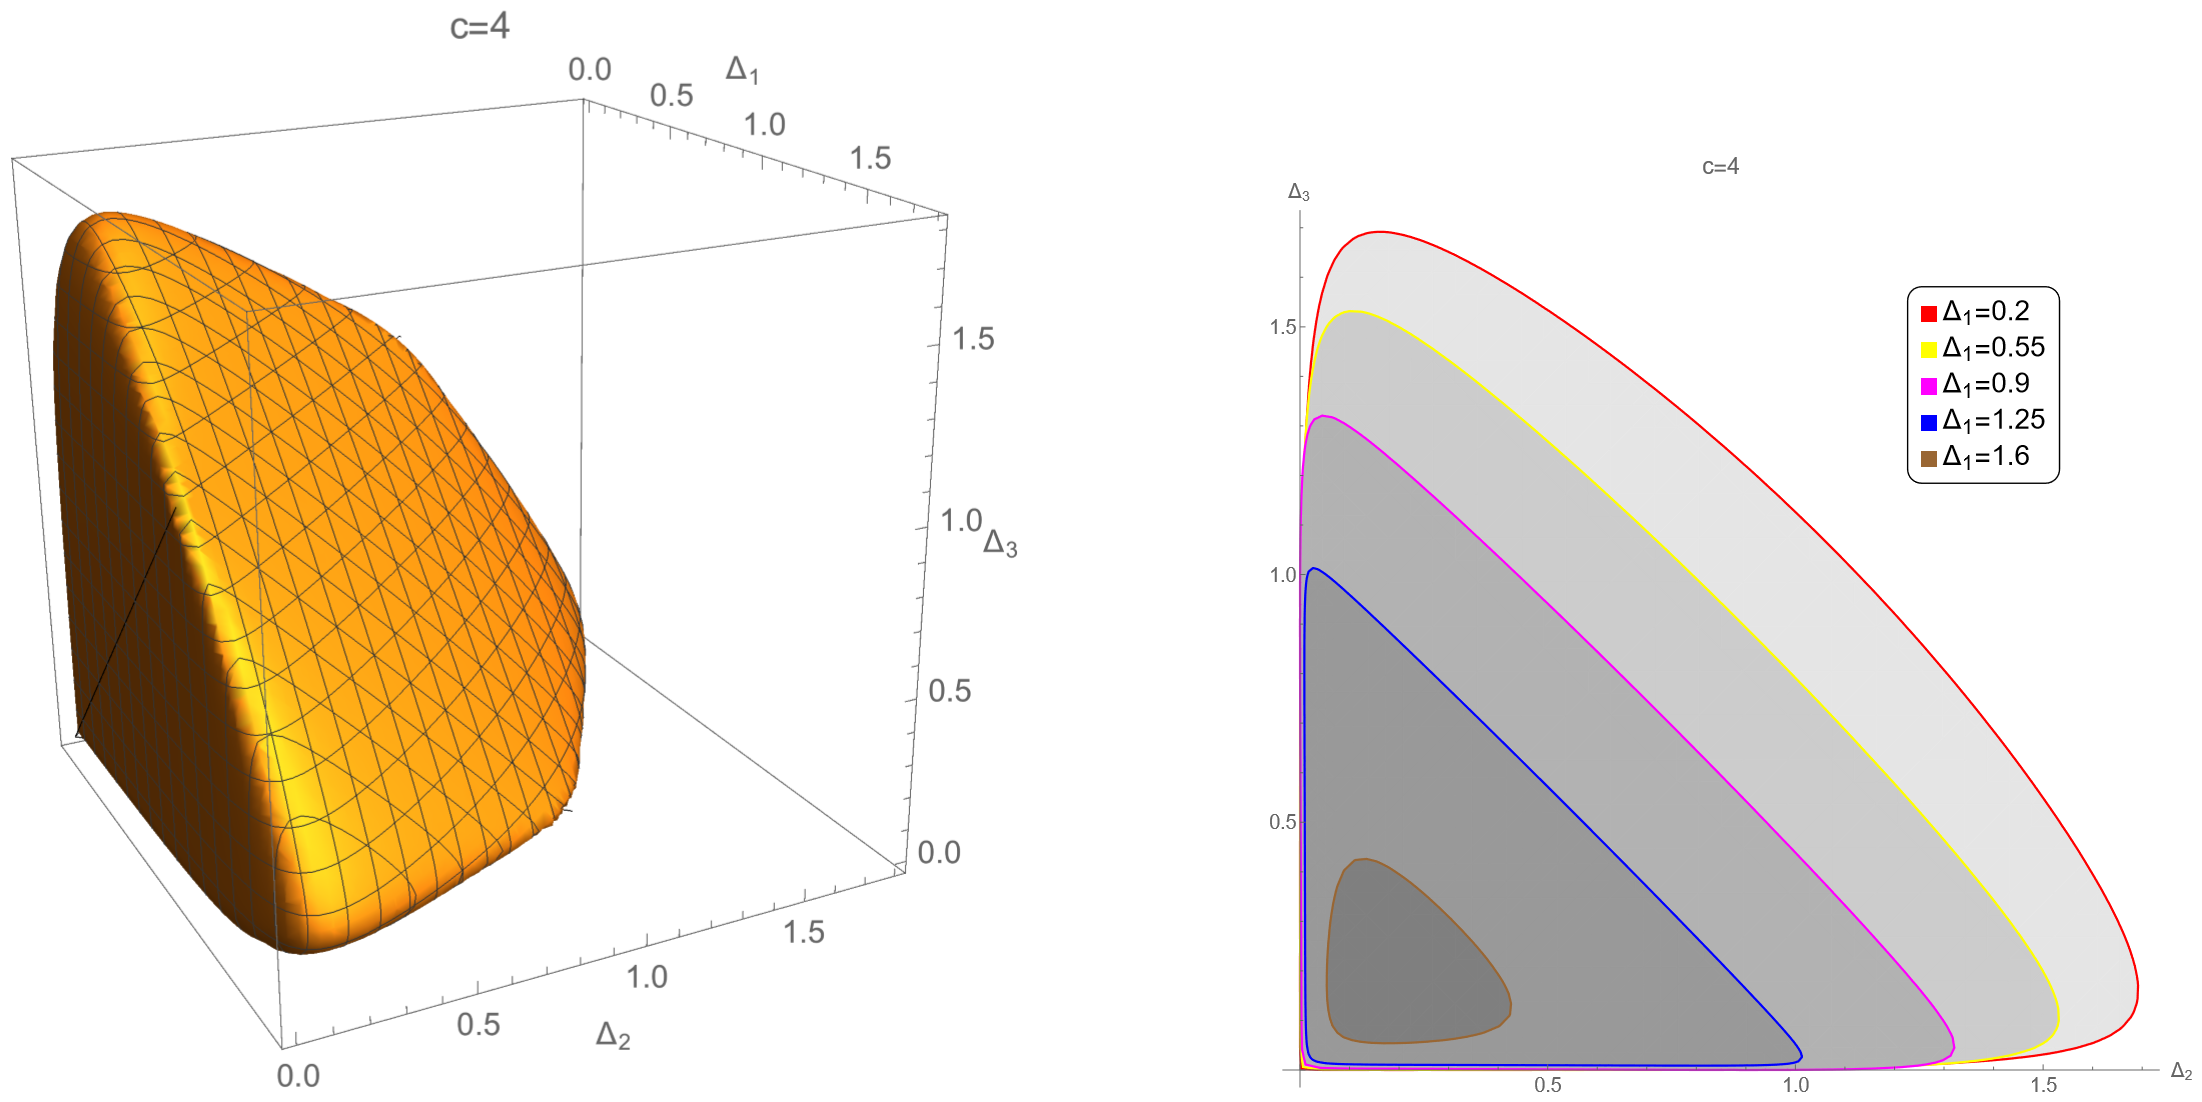
\includegraphics[width=0.85\textwidth]{figures/fig21.png}
  \caption{左：$c=4$ 时区域 $D_\Delta^{(3)}$ 的三维图。右：该区域在 $\Delta_1$ 取常数时的截面。图取自~\cite{r68}。（原文 p.49，图 21）}
  \label{fig:21}
\end{figure}

为偏离 Rényi 曲面，与其改变几何，不如在覆盖黎曼球面的三页中的任意一页插入能动张量 $T(z)$，或更一般的单位算符的 Virasoro 后代 $L_{-n_1}\cdots L_{-n_k}$。这样便能写出一般模的亏格二块在 Rényi 轨迹附近的展开，从而对 $C_{ijk}^2$ 表述完整的亏格二模交叉方程组。

% ===== 原书 p.48 末至 p.50（PDF 49--50）：第 6 章与致谢 =====

\section{总结}
\label{sec:6}

\begin{keytakeaways}
  \item 核心物理图像：可解的二维 CFT 仍局限于自由或有理理论、少数非紧致陪集模型及其轨形；一般二维 CFT 的完整自举方程组虽已写出，却仍无法实际求解。
  \item 使用的数学工具：交叉对称性与模不变性（环面一点函数的模协变、亏格二配分函数的模不变）给出的完整相容关系，以及半正定规划、线性泛函等数值手段。
  \item 本节结论：要刻画一般二维 CFT，必须把大量原初的 OPE 与模协变约束组织成具有正性的方程组（如亏格二模自举）；对非有理、紧致、相互作用的 CFT，目前的构造能力仍极为有限。
\end{keytakeaways}

过去四十年间，二维 CFT 方面积累了相当多的知识。然而，可解的二维 CFT 大体上仍局限于自由理论或有理理论、少数几个非紧致陪集模型，以及它们的轨形。

即便最简单的一类有理 CFT，即亚纯（meromorphic）CFT，也远未被分类：用配分函数的模不变性约束其谱很容易；但要证明存在一组结构常数，满足全部交叉方程与模协变的环面一点函数（不借助额外输入，例如对称性假设~\cite{r69}），却相当困难。

我们对相互作用、紧致、非有理 CFT 的了解少得令人难堪：唯一稳健的构造都基于 $(2,2)$ 超共形理论的精确边缘形变。迄今我们还不知道任何一个幺正、紧致 CFT 的例子，能在 Virasoro 对称性之外不含额外的高自旋守恒流。\footnote{临界耦合 Potts 模型~\cite{r54} 是一个潜在候选，但据我所知，它是否等价于某个已知的有理陪集模型，尚未被排除。}因此，要么我们漏掉了重要的约束（例如：$\frac{c-1}{12}$ 真的是扭曲间隙的最优上界吗~\cite{r58}？），要么我们对一般的二维 CFT 长什么样毫无头绪。显然，我们才刚刚开始开辟二维 CFT 的版图，未来数十年还有大量东西要学。

% [Tutor Note: 正文把上界写作 $\frac{c-1}{12}$ 而不是 $\frac{c}{12}$：分子里的 $-1$ 使该界略低于 $c/12$，来自真空态（模不变真空特征标）的贡献；引用 \cite{r58} 时勿把分子写成 $c$。]

\section*{致谢}

感谢 TASI 2017 的组织者邀请我，也感谢参加的学生们的热情与富有启发性的问题。感谢 Chi-Ming Chang、Minjae Cho、Scott Collier、Petr Kravchuk、Ying-Hsuan Lin、Shu-Heng Shao、David Simmons-Duffin、Yifan Wang 的合作，以及 Thomas Dumitrescu、Daniel Harlow、Simeon Hellerman、Christoph Keller、Zohar Komargodski、Alex Maloney、Eric Perlmutter、Slava Rychkov、Ashoke Sen、Andy Strominger、Cumrun Vafa 的有益讨论。本工作由 Simons Foundation 的 Simons Investigator Award 与 DOE 基金 DE-FG02-91ER40654 支持。

% 以下为参考文献（References），由参考文献译者负责，本文件在此停止。
